%preamble
\documentclass[letterpaper]{article}
\synctex=1
\usepackage{graphicx}
\graphicspath{ {images/} }

\usepackage{lipsum}
\usepackage{float}
% \bibliographystyle{IEEEtran}
\bibliographystyle{ieeetr}

\usepackage{amssymb}
%actual document
\begin{document}

  % \maketitle %insert titlepage here
  \begin{titlepage}
    \begin{center}
        \vspace*{1cm}
        \Huge
        Experiment 1
        \vspace{1cm}

        Electrostatic Potentials and Fields
        \vspace{1cm}

        By: Arun Woosaree
        \vspace{1cm}

        Lab partners:
        \vspace{.25cm}
        \Large

        Fatemeh Ghafari Far

        Yvonne Hong
        \vspace{1cm}

        \Huge
        PHYS 230 Lab EH71
        \vspace{1cm}

        TA: Andrei Tetriakov
        \vspace{1cm}

        Date of Lab: \today
        \vfill
    \end{center}
\end{titlepage}

\section{Introduction}
% Begin with experiment’s objectives\\
% Give physical background:\\
% ○ Describe investigated/used\\
% phenomena e.g. Gauss’s law,\\
% field lines, equipotential lines.\\
% ○ Do not copy text from a
% textbook/manual\\
% Provide equations you used\\
% ○ Identify all symbols\\

In this experiment, we explore Gauss's Law using a circular capacitor, and
we map electric potential and the electric field of a parallel plate capacitor.
A capacitor is essentially two charged conductors separated by some insulator.
In Part 1, we measure the potential differences in the region between the charged conductors in a circular capacitor,
and since our geometry is simple, the electric potential can be compared with
predictions made using Gauss's Law. In Part 2, we make a contour map consisting of equipotential
curves from our data, which can then be used to construct the corresponding electric field lines
of the parallel plate capacitor.
By analyzing field patterns, we can determine the charge distribution on the surface of
the charged conductors.

The electric field \textbf{E} is defined such that a positive test charge $q$
placed in the electric field will experience a force $\textbf{F}=q\textbf{E}$.
Additionally, a certain amount of work $W=F \Delta s=qE\Delta s$ is done to move the charge
a distance $\Delta s$, parallel to the electrostatic force. The electrostatic force is
conservative, so the potential energy $U$ must decrease by $\Delta U=-qE\Delta s$.
$V$, the electric potential is defined to be potential energy per unit charge $V=U/q$.
The magnitude of an electric field at a point can be related to $V$ by
\begin{equation}
  E=-\frac{\Delta V}{\Delta s} \label{eq1}
\end{equation}

Using Gauss's law, in part 1 of the experiment we imagine a Gaussian cylinder enclosing
the inner and outer conductors of a circular capacitor. This cylinder has a radius $r$ and
length $L$ with flat end caps. Since \textbf{E} is parallel to the end caps, the flux, denoted $\Phi$ on
the end caps are zero, which leaves the curved surface of the cylinder, with area $2\pi rL$.
Since \textbf{E} is constant and perpendicular to the curved surface, the total flux $\Phi_E$ can be found
\begin{equation}
  \Phi_E = \Phi_{end1} + \Phi_cylinder + \Phi_{end2} = 0+E(2\pi rL) + 0 =\frac{Q}{\epsilon_0}
\end{equation}
\begin{figure}[H]
    \centering
    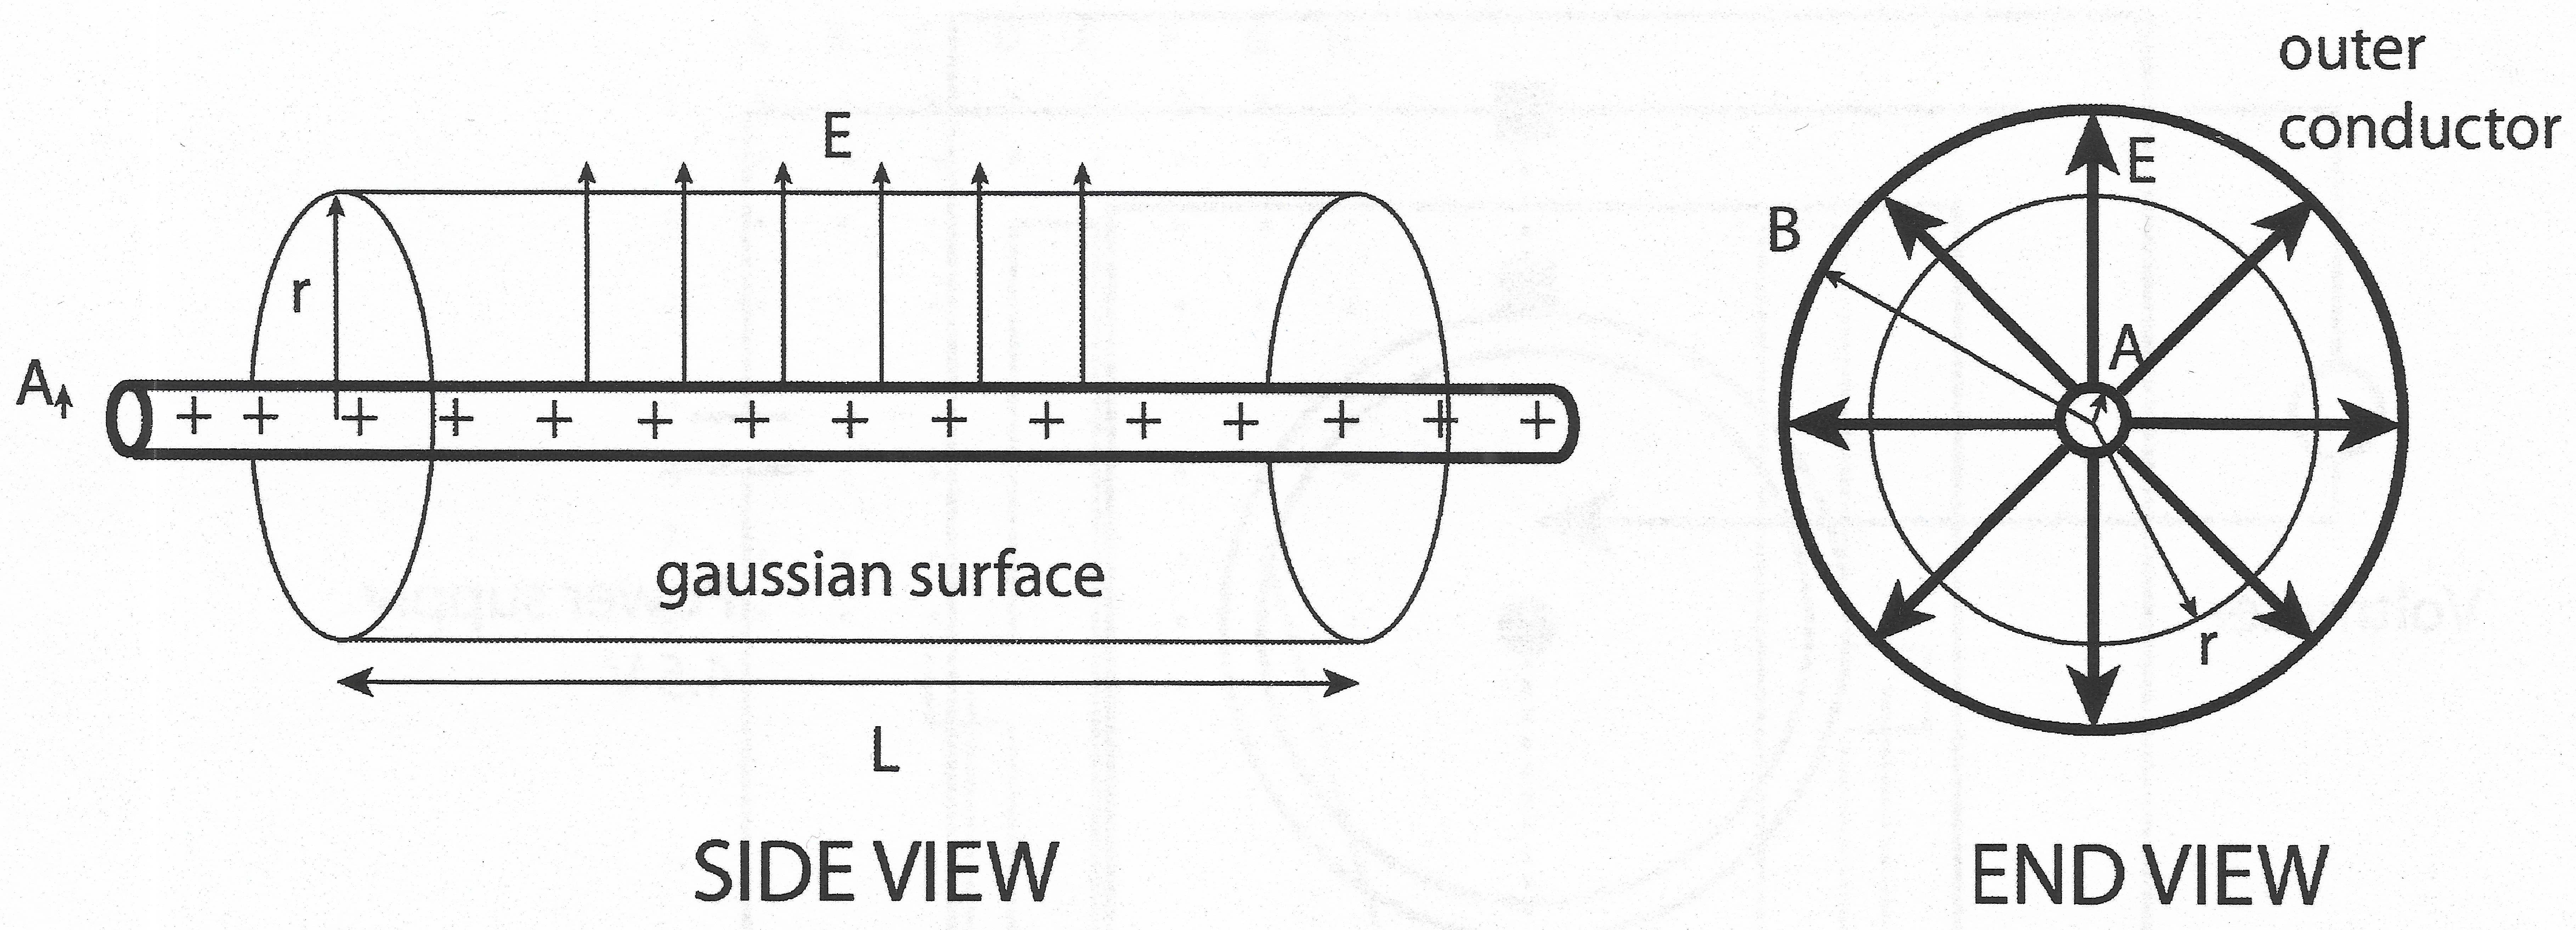
\includegraphics[width=\textwidth]{fig1.jpg}
    \caption{Gaussian Surface between two circular conductors. \cite{labmanual}}
\end{figure}

$\sigma$ is defined as the charge per unit area on the surface of the inner conductor.
The enclosed charge $Q$ enclosed by the Gaussian cylinder is $Q=(2 \pi AL)\sigma$, where
$A$ is the radius of the inner conductor, and $\epsilon_0=8.85418782 \times 10^{-12} m^{-3} kg^{-1} s^{4} A^{2}$ is the permittivity of free space.
Given the above information, the magnitude of the electric field at some radius $r$
can then be computed

\begin{equation}
  E=\frac{\sigma A}{\epsilon_0 r}
\end{equation}

If we put a probe at radius $r$, and the outer conductor has a radius $B$ then the voltage
difference between the probe and the outer conductor is
\begin{equation}
  V_r-V_B=\frac{\sigma A}{\epsilon_0 r} \ln{\frac{B}{r}}
\end{equation}
From which we can obtain the following equation if we set the voltage difference between the two conductors to have a value $V_0$
\begin{equation}
  \frac{V_r-V_B}{V_0}=\frac{\ln{\frac{B}{r}}}{\ln{\frac{B}{A}}}
\end{equation}
or alternatively,
\begin{equation}
  \ln{r} =\ln{\frac{A}{B}}(\frac{V_r-V_B}{V_0}) + ln{B}
\end{equation}
In part 2 of the experiment, we map the electric field of a parallel plate capacitor, and draw equipotential lines
which correspond to electric field lines. An equipotential surface is defined such that the
potential difference is constant at any point on the surface.


\section{Experimental Method}
% List all equipment used\\
% ○ Provide parameters as detailed as
% possible: masses, frequencies,
% etc.\\
% Report what YOU DID to achieve
% experimental goals:\\
% ○ Do not use imperative clause\\
% ○ Use first person narrative or
% passive voice\\
% Based on this section you should be
% able to reproduce your results without a
% manual

\textbf{List of Equipment:}
\begin{itemize}
  \item Circular capacitor (Figure 2)
  \item Parallel plate capacitor (Figure 3)
  \item Power Supply
  \item Voltmeter
\end{itemize}
For both parts of the experiment, the power supply was set to 4.5V. \\This is $V_0$ in equations 5 and 6.
\newpage
\subsection{Part 1}
In Part 1 of the experiment, a circuit was constructed using the above materials, as shown in the Figure 2 below.
The positive lead of the power supply was connected to the center of the circular capacitor, and the negative lead
was connected to the negative end on the voltmeter, and a probe was attached to the positive end of the voltmeter.
The probe was then touched at various radii on the circular capacitor, and the measured voltages were recorded in
a spreadsheet. The data was then plotted as the natural log of radius $r$ versus the voltage difference at radius $r$
to produce a linear graph. (Figure 4) The inner radius $A$ and outer radius $B$ as seen in Figure 1 were measured in centimetres, with a ruler
that had millimetre markings.
\begin{figure}[H]
    \centering
    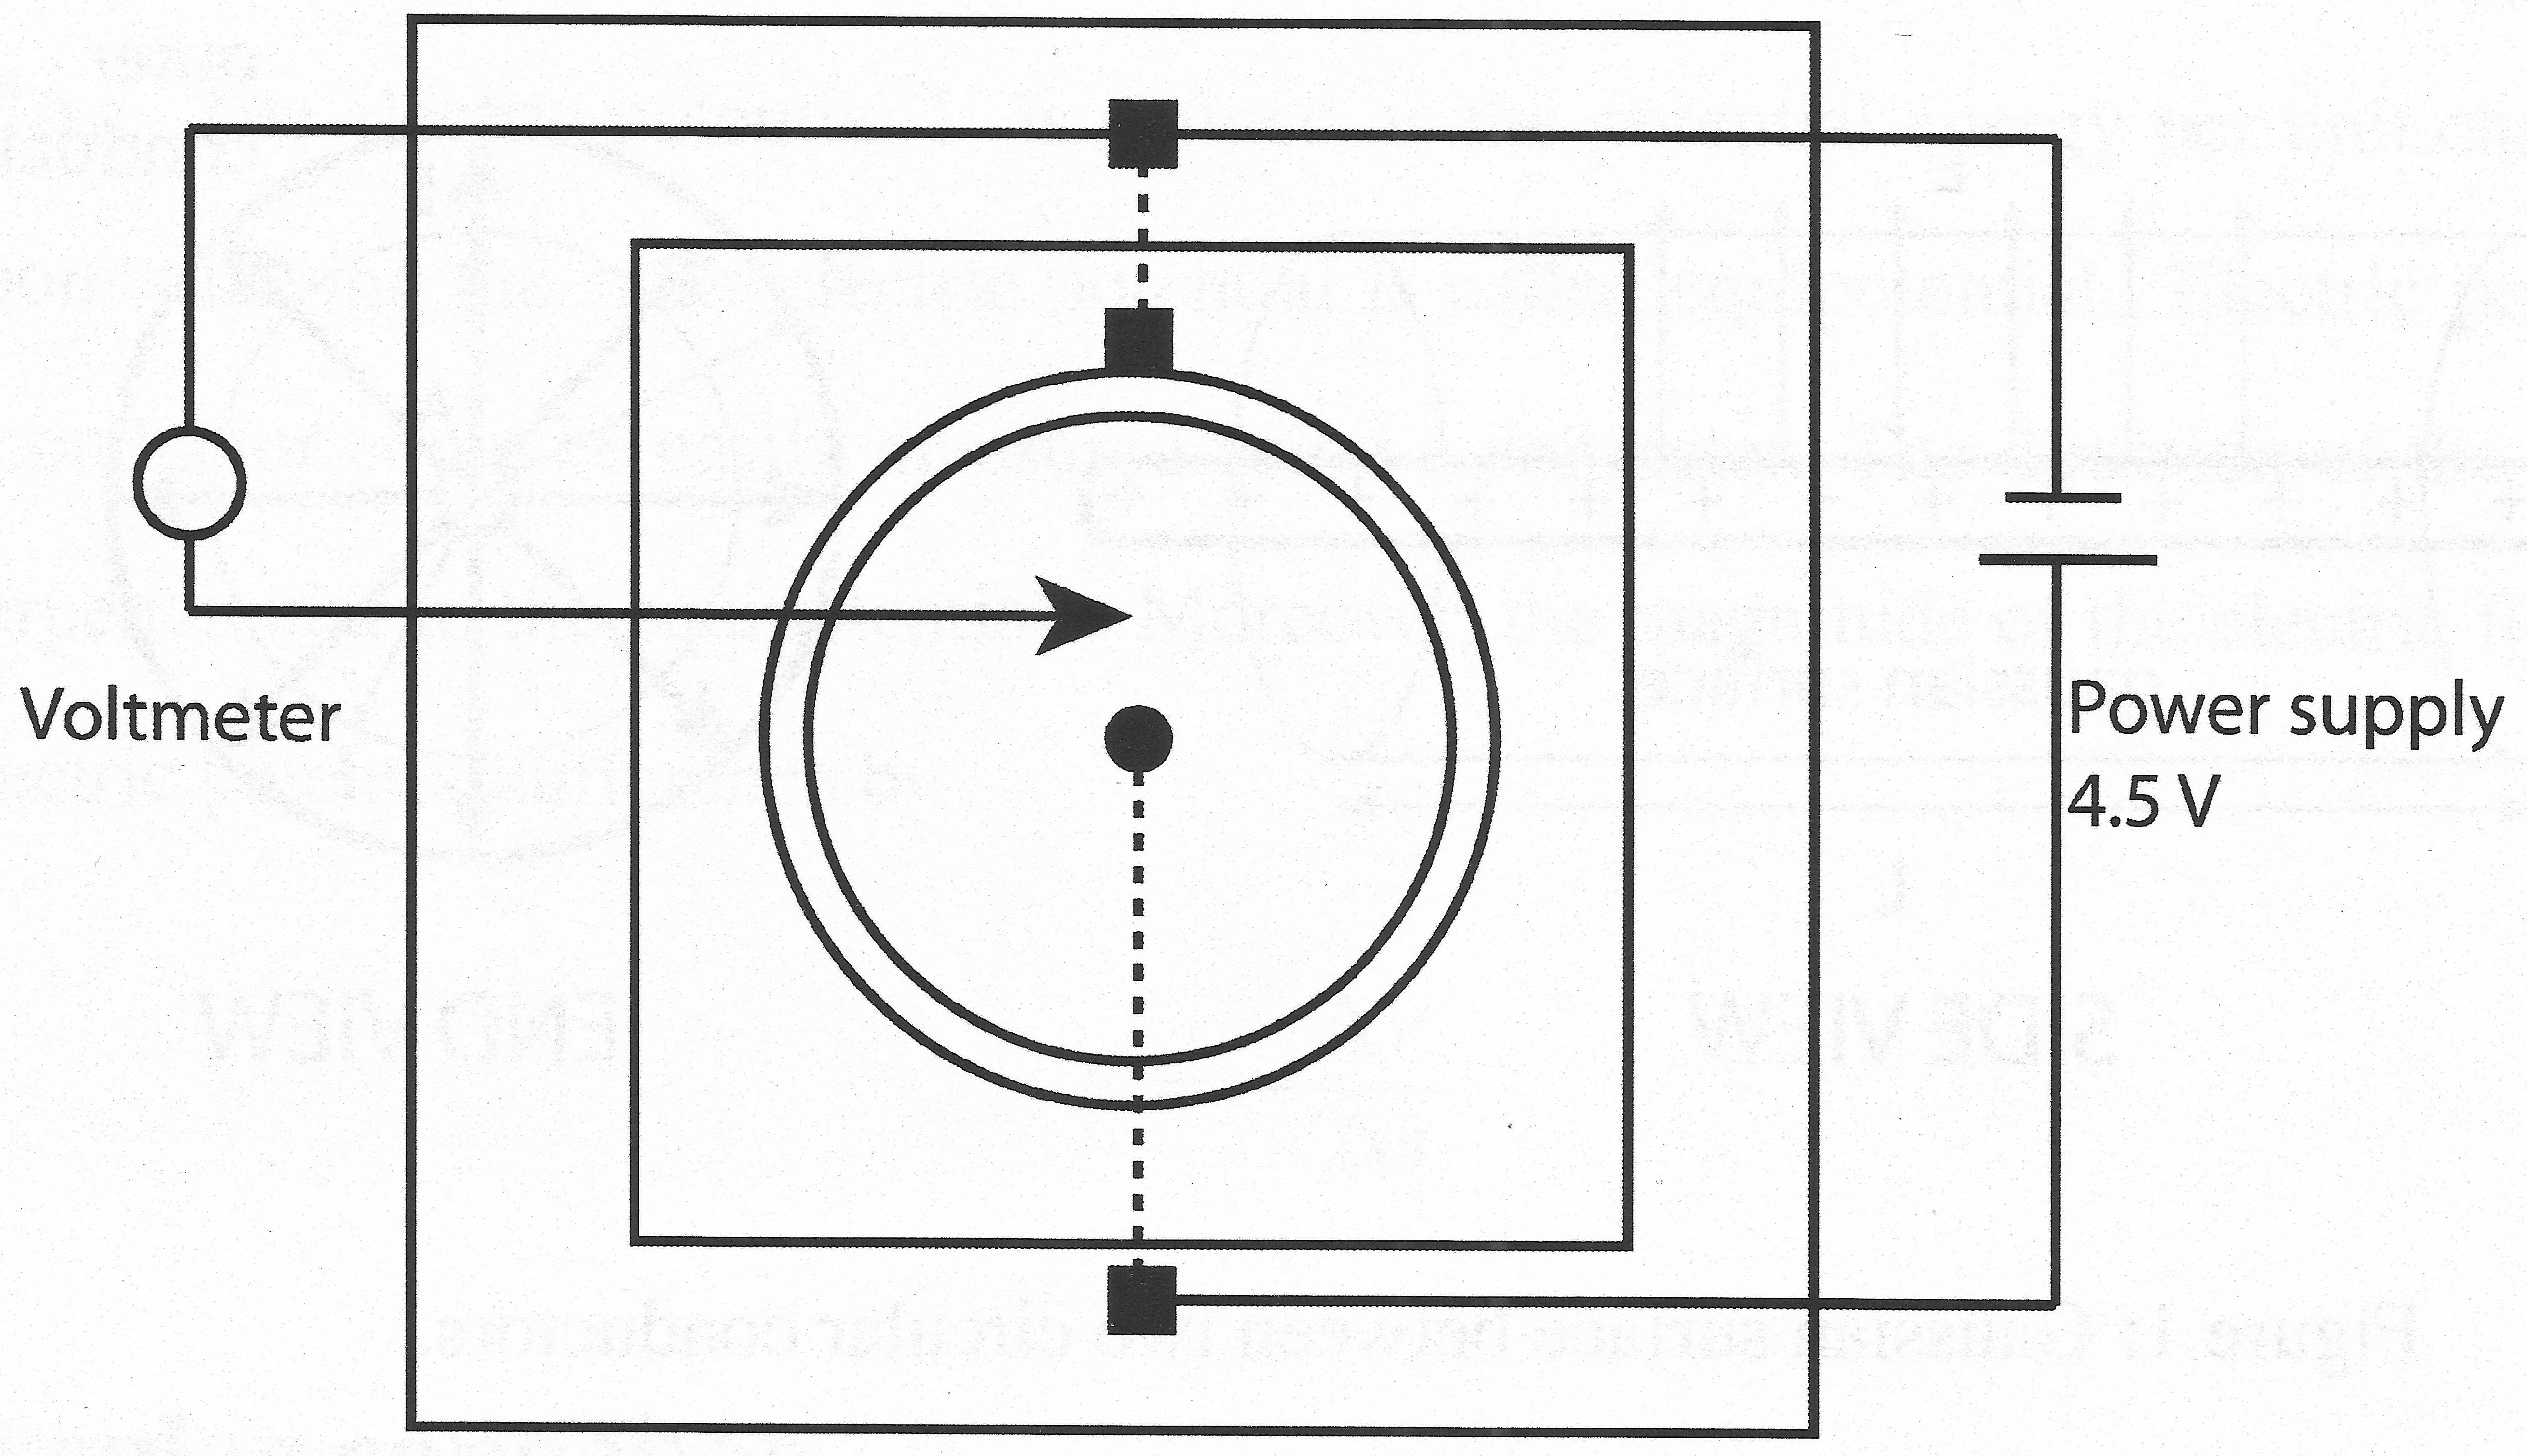
\includegraphics[width=.9\textwidth]{fig2.jpg}
    \caption{Measuring the voltage difference at various radii $r$ between two circular conductors. \cite{labmanual}}
\end{figure}


\subsection{Part 2}
In Part 2 of the experiment, a circuit was constructed using the parallel plate capacitor.
The positive end of the power supply was connected to one plate of the capacitor, and the negative
lead of the power suppply was connected to the side of the capacitor with markings for measuring potential
differences, and the negative end of the voltmeter. The probe remained connected to the positive end of the
voltmeter, as in Part 1. Once again, the probe was touched at various points on the capacitor, and the
voltage differences were recorded in a spreadsheet, from which Figures 5 and 6 were produced.

\begin{figure}[H]
  \centering
  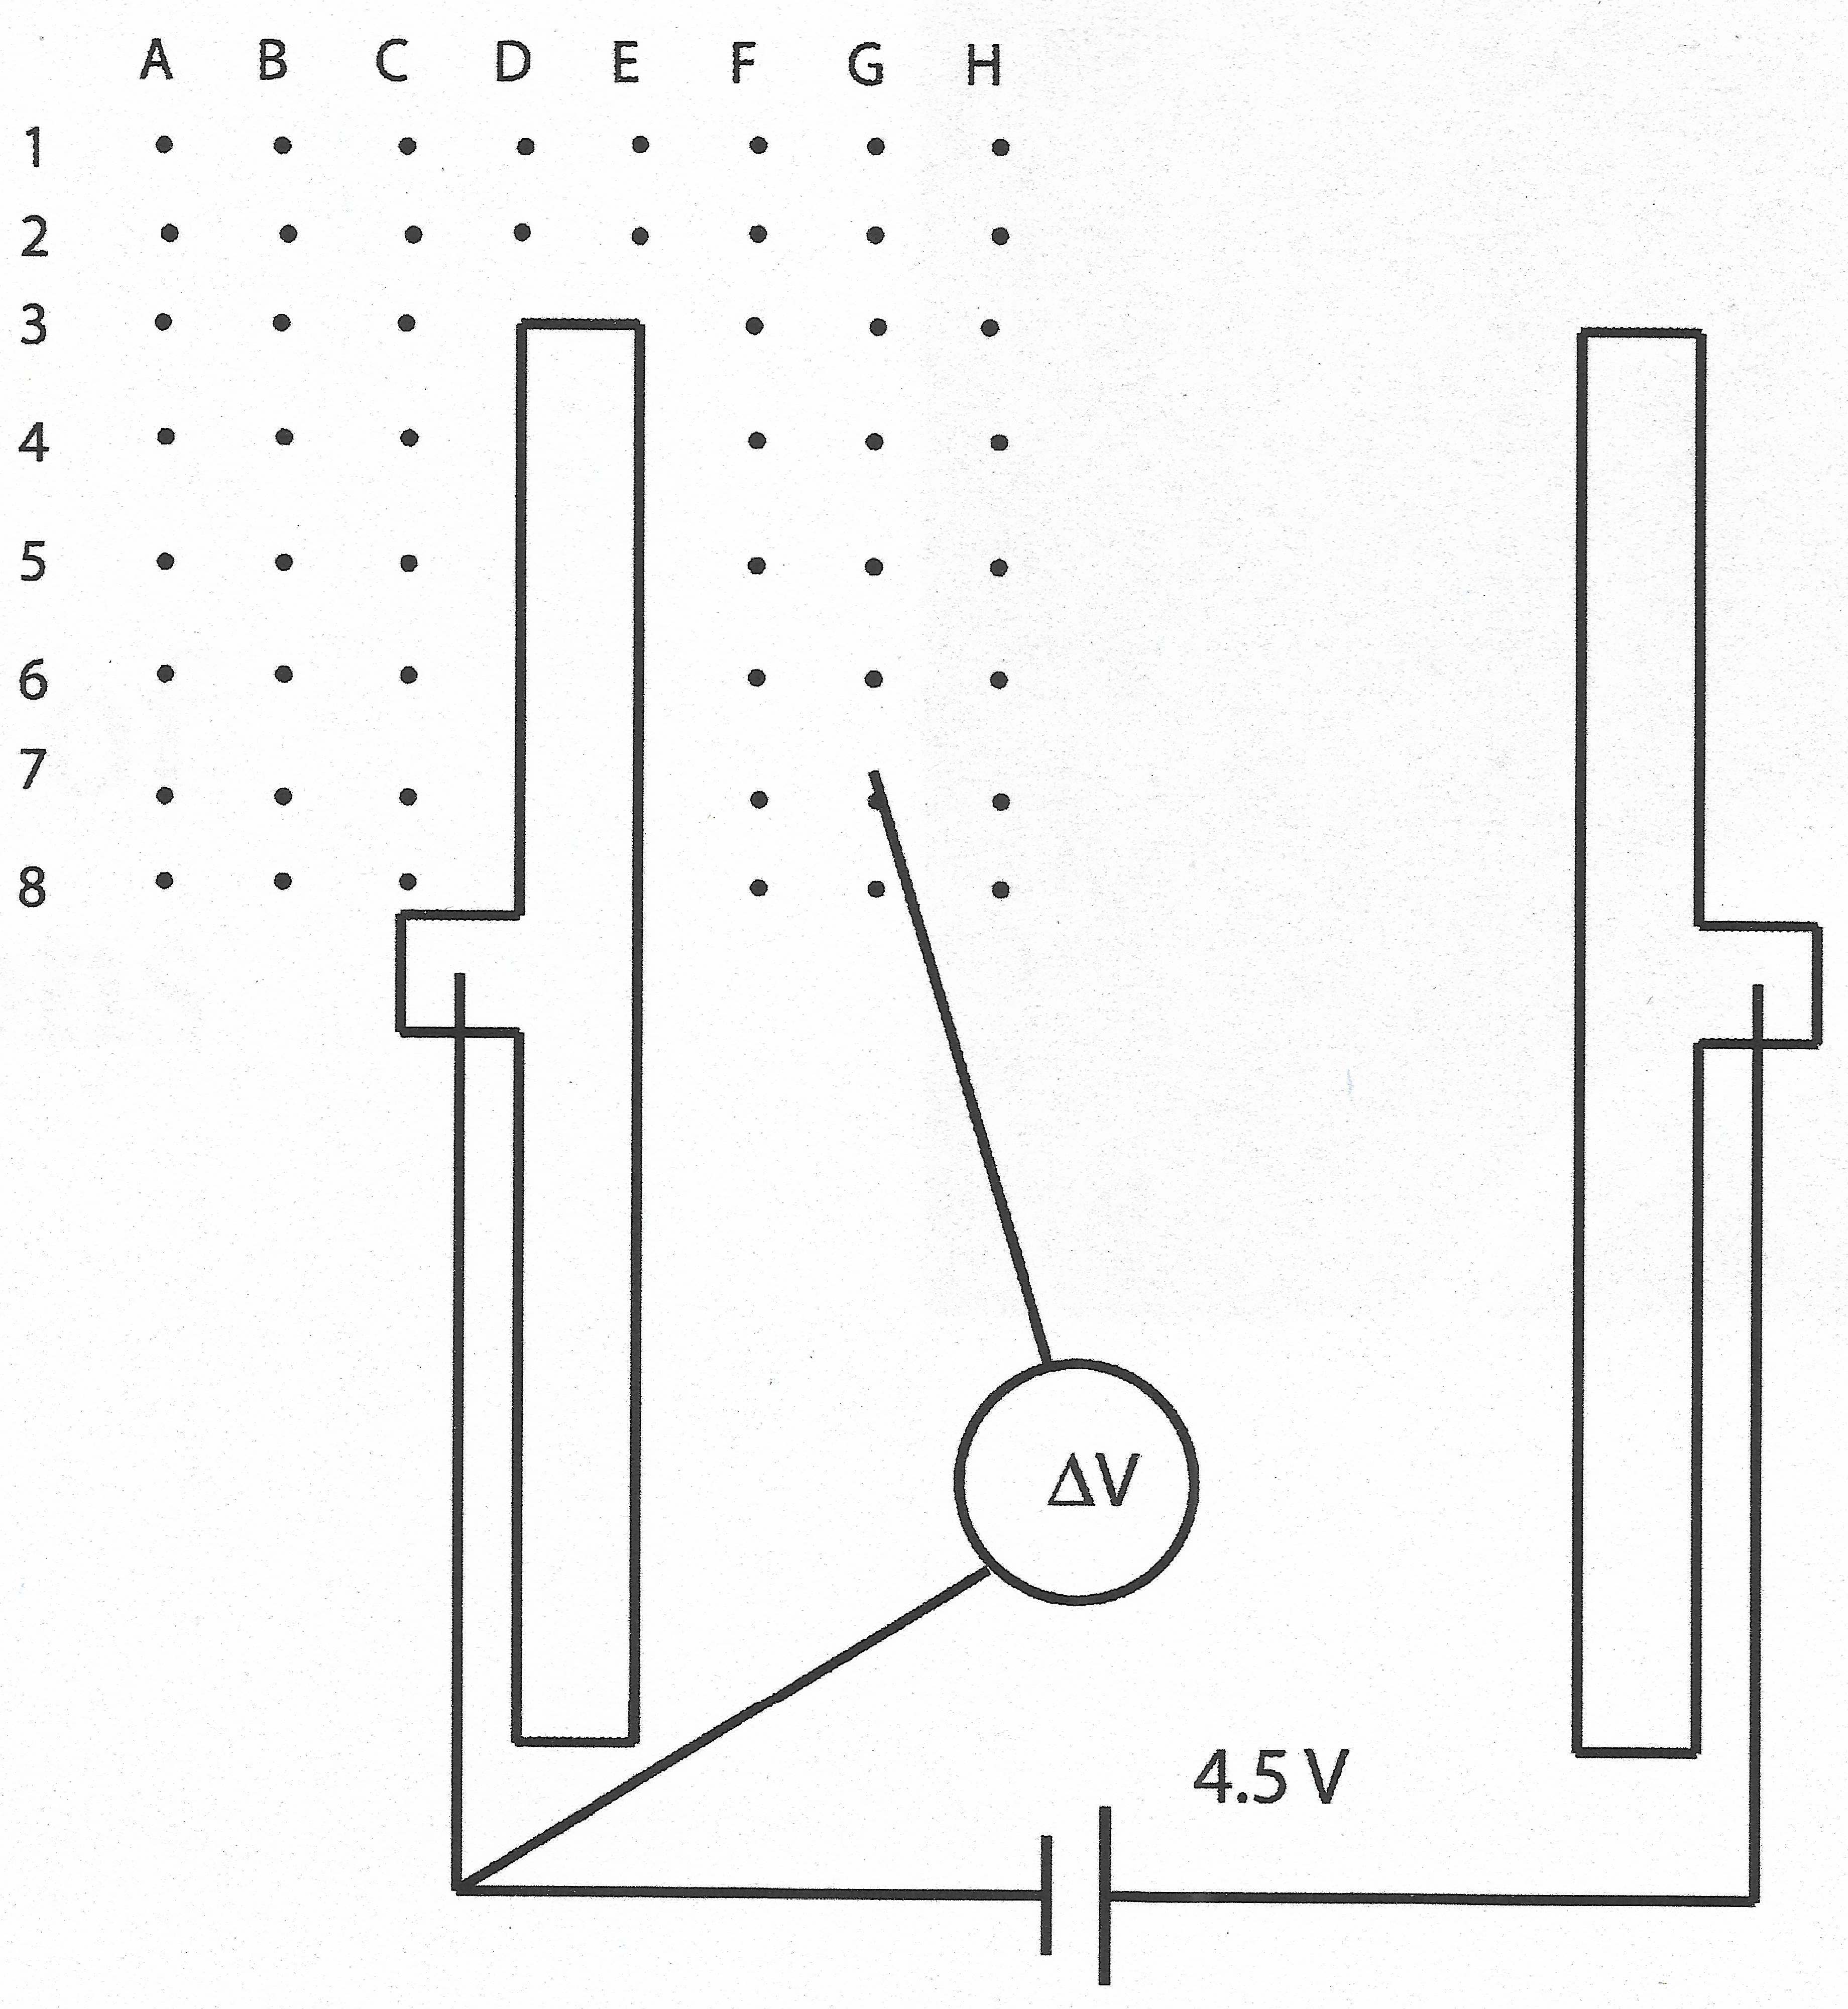
\includegraphics[width=.7\textwidth]{fig3.jpg}
  \caption{Measuring the voltage difference in a region between two parallel conductors. \cite{labmanual}}
\end{figure}

% When the apparatus illustrated above is set up, i.e. the lengths ‘r’ and ‘R’ are known, the center of the spark tape is marked when the bob is hanging freely at rest, and the bob is at the starting position, being held by the electromagnet, and the string is steadied to lessen any vibrations, the power going to the electromagnet is cut, and as a result, the bob is released from rest. The ‘RUN’ button on the spark timer is immediately (as best as humanly possible) held down, until the bob reaches approximately the maximum height on the other side of the track, or when one half of the period of the pendulum is completed.
%
% The spark timer is set to spark 30 times a second, so the time elapsed between each burn hole on the spark tape is 1/30th of a second. Once the spark tape is obtained from the apparatus, we need to measure the displacements of the glider as it was moving. To do so, we use a meter stick, and a displacement of 0.00m is taken to be the at the center of the spark tape, which is the point that was marked while the bob hangs freely at rest. This means that the initial displacement of the bob is taken to be a negative displacement, and the points after the bob passes the center are taken to be positive.
%
% After measuring the displacements of the bob, we enter the data points into Excel, and also calculate the time elapsed for each data point. (Ex. At the 10th burn hole, the time elapsed would be 10*1/30 seconds). From this data, we can calculate EK , EP , and ET  using equations  5,9 and 10 and plot them on a graph as a function of time. The ET curve was fit to a linear regression, and the EK and EP curves were fit to quadratic curves.

\section{Results}


% Should be a coherent text\\
% Present all data and calculations with words. Examples:\\
% ○ “Row data for free-fall acceleration measurements is given by Table 1.”\\
% ○ “In order to find the acceleration we plot doulbed distance as a function of
% time squired as is shown by Figure 1.” or “To find the acceleration we
% linearize Equation 1 as d(x)=ax, where x=t2/2 and plot it on Figure 1”.\\
% ○ “The slope of the graph corresponds to the acceleration and can be found
% along with the uncertainty using LINEST(see Table 2)”\\
% ○ “The uncertainty in distance is calculated as d= x+ y”\\
% ○ “Finally, the acceleration due to gravity is 9.81± 0.03 m/s2 ”\\
% All figures and should have label and caption \\(e.g. “Figure 1: position as a function
% of time during free fall”).\\
% Use scientific notation (103, not 1E3) and appropriate significant digits

\subsection{Part 1}
% Part I\\
% Linearized equation: provide
% all parameters e.g. variables,
% slope, intercept, etc.\\
% Linear graph: add trendline,
% provide fitting parameters
% (slope, intercept)\\
% Give values A and B obtained
% from the graph and measured
% directly\\
% Use Linest to find
% uncertainties\\

Raw data recorded while measuring potential differences at various radii on
the circular capacitor is given by Table 1.
\begin{table}[H]
\centering
\begin{tabular}{|c|c|}
\hline
 Radius $r$ (cm) & Voltage (V)\\ \hline
 2.5         & 3.45        \\ \hline
 3           & 3.03        \\ \hline
 3.5         & 2.63        \\ \hline
 4           & 2.27        \\ \hline
 4.5         & 1.89        \\ \hline
 5           & 1.72        \\ \hline
 5.5         & 1.49        \\ \hline
 6           & 1.26        \\ \hline
 6.5         & 0.86        \\ \hline
 7           & 0.62        \\ \hline
 7.5         & 0.59        \\ \hline
 8           & 0.45        \\ \hline
 8.5         & 0.2         \\ \hline
\end{tabular}
\caption{Raw data recorded when measuring potential differences at various radii $r$ on the circular capacitor.}
\end{table}

Using the data in Table 1, a linear graph is generated by taking the natural logarithm of the
radii, and setting $\ln{(r)}$ to be the y-axis. The potential difference is then divided by $V_0=4.5 V$
and plotted on the x-axis. As a result, by observing Equation 6, we can see that the
slope of the graph is $\ln{\frac{A}{B}}$, and the y-intercept is $\ln{(B)}$
\begin{figure}[H]
  \centering
  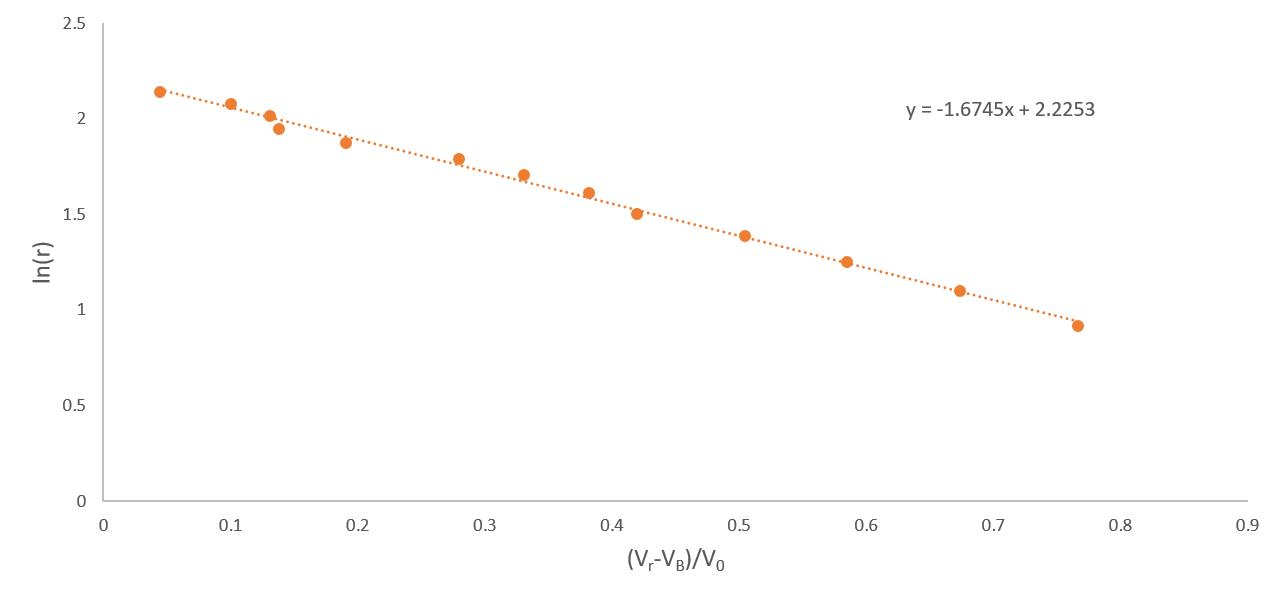
\includegraphics[width=\textwidth]{chart1.png}
  \caption{Measuring the voltage difference in a region between two parallel conductors.}
\end{figure}
\newpage
Using Excel's LINEST function, we can obtain the following data from the graph in Figure 4.
\begin{table}[H]
\centering
\begin{tabular}{cc}
  Slope  $\ln{\frac{A}{B}}$ &  $-1.674456326\pm0.03399955317$ \\
  Y-Intercept $\ln{(B)}$   &  $2.225330849\pm0.01408922355$ \\
\end{tabular}
\caption{LINEST data from the graph in Figure 4}
\end{table}


From our LINEST data (Table 2), we can see that the y-intercept $\ln{(B)}=2.22533084879698$
Thus, the calculated value of $B$ from the graph can be found by exponentiating $\ln{(B)}$.\\
  $$B= e^{ln(B)} = e^{2.22533084879698}=9.25654481406370...$$
And the error $\delta B$ can be calculated:
$$ \delta \ln{(B)} = \frac{\delta B}{|B|}$$
$$ \therefore \delta B = \delta \ln{(B)} \times |B| = 0.01408922355 \times 9.25654481406370 = 0.13041752...\approx 0.1  $$
So, $B=9.3\pm 0.1 cm$ is the value for inner radius $B$ obtained from the graph.
The percent error is:
$$ \frac{|9.25654481406370-9.5|}{9.5}\times100 = 2.56\%$$

\noindent To obtain the calculated value for $A$, we can see from our LINEST data (Table 2) that the slope $\ln{\frac{A}{B}}=-1.674456326$
Thus, the calculated value of $A$ can be found
$$ e^{\ln{\frac{A}{B}}}=e^{-1.674456326} = \frac{A}{B} = 0.1874100418... $$
$$ A= B \times \frac{A}{B} = 9.25654481406370 \times 0.1874100418 = 1.73476945...$$
And the error can be calculated:
$$ \delta \ln{\frac{A}{B}} =\frac{\delta{\frac{A}{B}}}{|\frac{A}{B}|}  $$
$$ \therefore \delta \frac{A}{B} = \delta \ln{\frac{A}{B}} \times \left|{\frac{A}{B}}\right| = 0.03399955317 \times 0.1874100418 = 0.0063718...$$
$$ \delta \frac{A}{B} = \left|\frac{A}{B}\right|\left(\frac{\delta A}{|A|}+\frac{\delta B}{|B|}\right) $$
$$ \therefore \delta A = \left(\frac{\delta \frac{A}{B}}{|\frac{A}{B}|} - \frac{\delta B}{|B|} \right)|A| = \left( \frac{0.0063718576}{0.1874100418} - \frac{0.13041752}{9.25654481406370} \right)
 1.73476945 = 0.03453983253...\approx 0.03$$

\noindent So, $A=1.73 \pm 0.03 cm$ is the value for outer radius $A$ obtained from the graph.
The percent error is:
$$ \frac{|1.73476945-1.9|}{1.9}\times100 = 8.70\%$$

\vspace{1cm}
\noindent The calculated values of $A$ and $B$ from the graph are summarized in Table 3.
\begin{table}[H]
\centering
\begin{tabular}{c|c|c|c|}
                & Measured            & Obtained from graph: & \% Error \\ \hline
Inner radius A: & $1.9 \pm 0.1 cm$      & $1.73 \pm 0.03 cm$           &    $2.56$  \\ \hline
Outer radius B: & $9.5 \pm 0.1 cm$      & $9.3 \pm 0.1 cm  $           &    $8.70$  \\ \hline
\end{tabular}
\caption{Measured values of $A$ and $B$ compared to the calculated values obtained from the graph.}
\end{table}

\subsection{Part 2}
% Part II\\
% Provide graph from the template\\
% By hand draw field lines, show charge
% distribution, etc.\\
% Provide the explanation, calculations,
% answer questions in Discussion.\\

Raw data recorded while measuring potential differences at various points on
the parallel plate capacitor is given by Table 4. Each cell corresponds to one
of the points on the grid as seen in Figure 3.

% Please add the following required packages to your document preamble:
% \usepackage{graphicx}
\begin{table}[H]
\centering
\resizebox{\textwidth}{!}{%
\begin{tabular}{l|l|l|l|l|l|l|l|l|l|l|l|l|l|l|l|l|}
   & A    & B    & C    & D    & E    & F    & G    & H    & H'   & G'   & F'   & E'   & D'   & C'   & B'   & A'   \\ \hline
1  & 0.51 & 0.60 & 0.71 & 0.92 & 1.14 & 1.38 & 1.72 & 2.30 & 2.20 & 2.78 & 3.12 & 3.36 & 3.58 & 3.79 & 3.90 & 3.99 \\ \hline
2  & 0.46 & 0.53 & 0.58 & 0.76 & 0.92 & 1.28 & 1.67 & 2.24 & 2.26 & 2.83 & 3.22 & 3.58 & 3.74 & 3.92 & 3.97 & 4.04 \\ \hline
3  & 0.40 & 0.42 & 0.43 & 0.46 & 0.60 & 1.09 & 1.62 & 2.16 & 2.34 & 2.88 & 3.41 & 3.90 & 4.04 & 4.07 & 4.08 & 4.10 \\ \hline
4  & 0.33 & 0.30 & 0.25 & 0.00 & 0.00 & 0.87 & 1.47 & 2.13 & 2.37 & 3.03 & 3.63 & 4.50 & 4.50 & 4.25 & 4.20 & 4.17 \\ \hline
5  & 0.27 & 0.22 & 0.14 & 0.00 & 0.00 & 0.78 & 1.42 & 2.06 & 2.44 & 3.08 & 3.72 & 4.50 & 4.50 & 4.36 & 4.28 & 4.23 \\ \hline
6  & 0.23 & 0.17 & 0.09 & 0.00 & 0.00 & 0.75 & 1.36 & 2.04 & 2.46 & 3.14 & 3.75 & 4.50 & 4.50 & 4.41 & 4.33 & 4.27 \\ \hline
7  & 0.21 & 0.14 & 0.08 & 0.00 & 0.00 & 0.79 & 1.37 & 2.03 & 2.47 & 3.13 & 3.71 & 4.50 & 4.50 & 4.42 & 4.36 & 4.29 \\ \hline
8  & 0.18 & 0.13 & 0.00 & 0.00 & 0.00 & 0.71 & 1.38 & 2.04 & 2.46 & 3.12 & 3.79 & 4.50 & 4.50 & 4.50 & 4.37 & 4.32 \\ \hline
9  & 0.16 & 0.10 & 0.00 & 0.00 & 0.00 & 0.71 & 1.29 & 2.05 & 2.45 & 3.21 & 3.79 & 4.50 & 4.50 & 4.50 & 4.40 & 4.34 \\ \hline
9' & 0.16 & 0.10 & 0.00 & 0.00 & 0.00 & 0.71 & 1.29 & 2.05 & 2.45 & 3.21 & 3.79 & 4.50 & 4.50 & 4.50 & 4.40 & 4.34 \\ \hline
8' & 0.18 & 0.13 & 0.00 & 0.00 & 0.00 & 0.71 & 1.38 & 2.04 & 2.46 & 3.12 & 3.79 & 4.50 & 4.50 & 4.50 & 4.37 & 4.32 \\ \hline
7' & 0.21 & 0.14 & 0.08 & 0.00 & 0.00 & 0.79 & 1.37 & 2.03 & 2.47 & 3.13 & 3.71 & 4.50 & 4.50 & 4.36 & 4.36 & 4.29 \\ \hline
6' & 0.23 & 0.17 & 0.09 & 0.00 & 0.00 & 0.75 & 1.36 & 2.04 & 2.46 & 3.14 & 3.75 & 4.50 & 4.50 & 4.41 & 4.33 & 4.27 \\ \hline
5' & 0.27 & 0.22 & 0.14 & 0.00 & 0.00 & 0.78 & 1.42 & 2.06 & 2.44 & 3.08 & 3.72 & 4.50 & 4.50 & 4.36 & 4.28 & 4.23 \\ \hline
4' & 0.33 & 0.30 & 0.25 & 0.00 & 0.00 & 0.87 & 1.47 & 2.13 & 2.37 & 3.03 & 3.63 & 4.50 & 4.50 & 4.25 & 4.20 & 4.17 \\ \hline
3' & 0.40 & 0.42 & 0.43 & 0.46 & 0.60 & 1.09 & 1.62 & 2.16 & 2.34 & 2.88 & 3.41 & 3.90 & 4.04 & 4.07 & 4.08 & 4.10 \\ \hline
2' & 0.46 & 0.53 & 0.58 & 0.76 & 0.92 & 1.28 & 1.67 & 2.24 & 2.26 & 2.83 & 3.22 & 3.58 & 3.74 & 3.92 & 3.97 & 4.04 \\ \hline
1' & 0.51 & 0.60 & 0.71 & 0.92 & 1.14 & 1.38 & 1.72 & 2.30 & 2.20 & 2.78 & 3.12 & 3.36 & 3.58 & 3.79 & 3.90 & 3.99 \\ \hline
\end{tabular}%
}
\caption{Raw data recorded when measuring potential differences at various points on the parallel plate capacitor.}
\end{table}
\newpage
From the above data, the following graph was generated in Figure 5, which gives a visual representation of the electric
equipotential lines on the capacitor.

\begin{figure}[H]
  \centering
  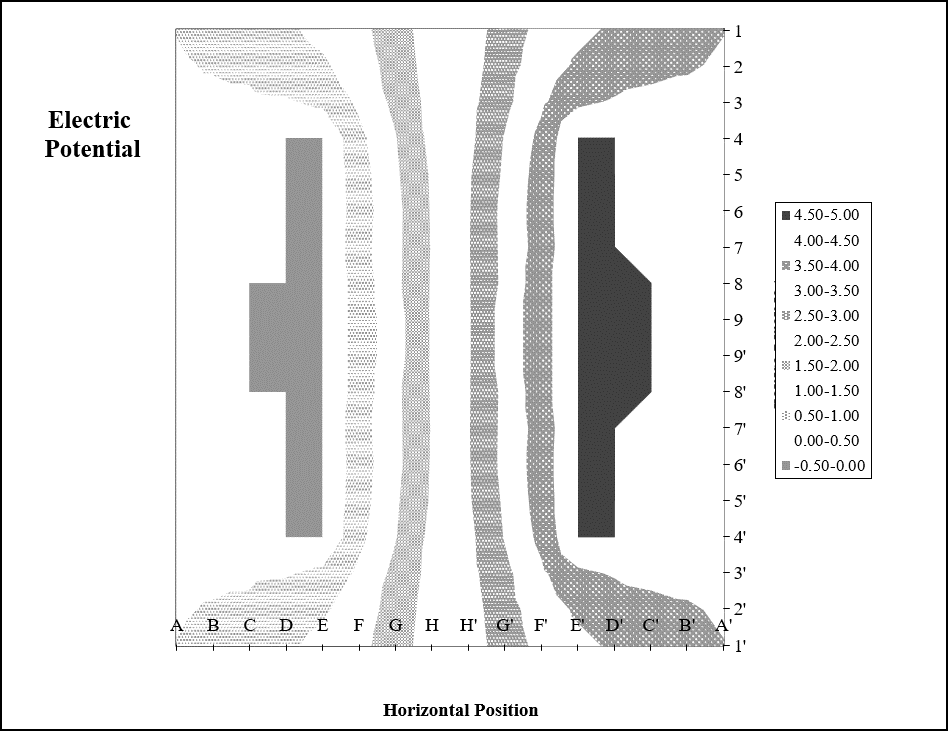
\includegraphics[width=.9\textwidth]{chart2.png}
  \caption{A visual representation of the electric equipotential lines between the plates of the capacitor. This figure was generated using the data in Table 4.}
\end{figure}
\vspace{2cm}
The next figure, (Figure 6) was also generated from the data in Table 4, which is a 3
dimensional plot of the potential difference at different points on the parallel plate capacitor
as a function of the horizontal and vertical positions of the probe.
\begin{figure}[H]
  \centering
  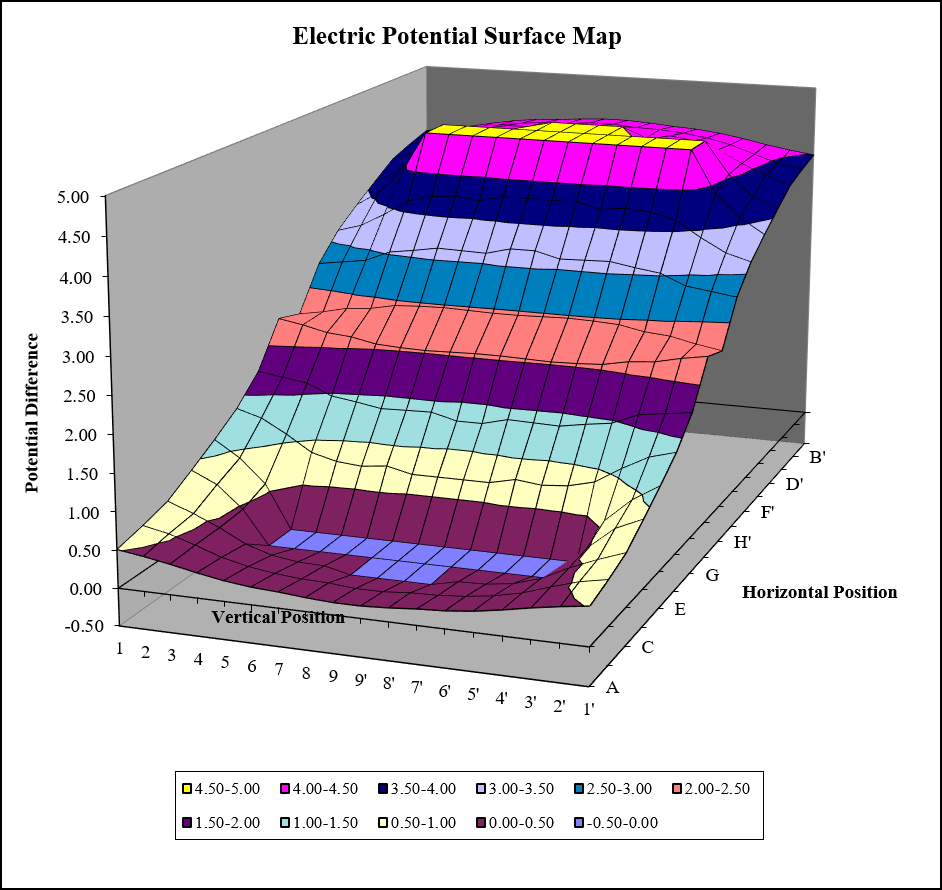
\includegraphics[width=\textwidth]{chart3.png}
  \caption{An electric potential surface map generated from the data in Table 4 above}
\end{figure}



\section{Discussion}

\subsection{Part 1}
From Table 3, we can see that our calculated values for the inner radius A
($1.73 \pm 0.03 cm$)
and outer radius B
($9.3 \pm 0.1 cm$) were fairly close to the measured values $1.9 \pm 0.1 cm$ for A
and $ 9.5 \pm 0.1 cm$ for B.
Additionally, the percent error did seem relatively good, being 2.56\% for A and 8.70\% for B.
Unfortunately, since $1.73$ does not fall within $1.9 \pm 0.1$,
and also since $9.3$ is not within $9.5 \pm 0.1$, our calculated values do not
agree within error of our measured values for A and B.

At first glance, the graph (Figure 4) produced from our raw data (Table 1) seems reasonable, especially
because all the data points recorded seem to fit nicely on the trendline with
no anomalous data points compared to the other values. This means that whatever error
introduced in our measurement of voltages was a constant factor, since we took care
to measure distances precisely, but relied on the voltmeter for recording voltages.
It is possible that the voltmeter was miscalibrated, resulting in readings that were slightly off,
since that would cause us to have potentially set the output voltage of the power supply $V_0$ from being $4.5 V$ to something else,
and the potential differences $V_r-V_B$ measured would be altered by about the same factor. Additionally,
it should be noted that when measuring the potential differences, the values read on the voltmeter varied
wildly, and we had to take multiple measurements, as pressing the probe on the capacitor with varying pressures and
angles could change the measured potential difference. We did our best to keep these factors constant.

\subsection{Part 2}
From figure 5, we can see how the equipotential lines along the capacitor show that the
electric field close to the center of the parallel plate capacitor is almost uniform because they are almost parallel, and
how we get fringing effects towards the edges of the capacitor, which make the electric field non uniform
in that area. This aligns well with what we have learned so far in the lecture part of this course.
\\ \\
The magnitude of the electric field is strongest where the equipotential lines are the closest.\\
Using equation 1,
$$ E=-\frac{\Delta V}{\Delta s}= -\frac{0.87 V -0.00 V}{0.95\times 10^{-2} m} = -91.58 \:V/m $$
\\ \\
\textbf{Questions: }\\ \\
\textit{The value of the voltage V is consant along an equipotential line.
Is the value of the field strength E necessarily constant along an electric field line?}\\
\textbf{A:}
\textbf{DOUBLE CHECK THIS} No. In Figure 5, we can see that
the nearly parallel lines close to the center of the capacitor mean that the electric field E is constant.
However, towards the edges of the conducting plates (Top and bottom part in Figure 5), the equipotential lines
curve due to fringing effects. As a result, E is no longer constant, since the equipotential lines
are no longer parallel to each other. This means that if V is constant along an equipotential line,
E is not necessarily constant as well.\\ \\
\textit{Describe the effect of the radius of curvature of a conductor on the concentation of charges}\\
\textbf{A:}
The condition for electrostatic equilibrium is that no charges are moving. For conductors, this means
that electrons are pushed towards the surface. Consider one electron at the surface of the conductor.
If there is curvature, there will be a parallel force acting on the electron due to other neighbouring
electrons because of Coulomb's Law. Areas that have smaller radii of curvature, however, the
parallel force is smaller. The net effect is an accumilation of charges in regoins on the conductor with
smaller radii of curvature.

\section{Conclusions}
In Experiment 1, we first measure potential differences at various radii on a circular capacitor,
and use Gauss's Law to calculate the inner and outer radii of the capacitor. We then check these predictions
by physically measuring the inner and outer radii of the circular capacitor. Although our data seemed
fine, our calculations did not agree within error of the measured values. Our inner radius was calculated to be
$1.73 \pm 0.03 cm$, while our measured value was $1.9 \pm 0.1 cm$, and the outer radius of the circular capacitor
was calculated as $9.3 \pm 0.1 cm$, while the measured value was $9.5 \pm 0.1 cm$. Since our resulting graph (Figure 4)
was linear as expected. with no anomalous data points, the source of error was a constant factor, and therefore can
likely be attributed to a faulty voltmeter. It should also be noted that when measuring the potential differences, pressing
the probe on the capacitor with varying pressures and angles could change the measured potential difference.
We did our best to keep these factors constant by taking multiple measurements.

Next, we measured potential differences at various points on a parallel plate capacitor, and used the data to generate
a graph which allows us to visualize the equipotential lines. The same data was also used to generate a 3 dimensional
plot of the potential differences as a function of the horizontal and vertical position of the probe on the parallel plate
capacitor. This allows us to visualize the electric potential on the capacitor.
  % In lab 8, we set up a pendulum with a 2.3kg bob hanging off of a string, and put an arced track such that the bob would be close enough to the track at any point while it swings to make a spark, with a spark timer. We then used an electromagnet to release the bob from rest, and used the spark timer to keep track of the bob’s displacements, and since the spark timer sparks at regular intervals, we had enough data to generate plots in Excel of potential energy, kinetic energy, and total energy as functions of time. The law of conservation of energy says that energy cannot be created or destroyed, but it can be converted. Theoretically, all of the Pe at the beginning should convert completely into KE, and then towards the end, all of the KE that the bob has should convert back into PE. Indeed, we do observe this behaviour in the lab, albeit not perfectly, since energy is also lost due to some of it being converted to other forms such as friction. This caused TE to decrease over time. Additionally, there were some anomalous data points that can be attributed to the spark timer missing sparks. Overall, however, the data seemed reasonable, albeit the amount of energy lost per second using the graph’s data versus taking an average after 25 periods did seem to disagree with 3 orders of magnitude.  One can observe the physics principles explored in the lab in real-life such as on a rollercoaster, where the gravitational potential energy is also converted into kinetic energy and vice versa such as when the car is going through a loop.
\bibliography{references}
\end{document}
